\documentclass[twoside]{book}

% Packages required by doxygen
\usepackage{fixltx2e}
\usepackage{calc}
\usepackage{doxygen}
\usepackage[export]{adjustbox} % also loads graphicx
\usepackage{graphicx}
\usepackage[utf8]{inputenc}
\usepackage{makeidx}
\usepackage{multicol}
\usepackage{multirow}
\PassOptionsToPackage{warn}{textcomp}
\usepackage{textcomp}
\usepackage[nointegrals]{wasysym}
\usepackage[table]{xcolor}

% Font selection
\usepackage[T1]{fontenc}
\usepackage[scaled=.90]{helvet}
\usepackage{courier}
\usepackage{amssymb}
\usepackage{sectsty}
\renewcommand{\familydefault}{\sfdefault}
\allsectionsfont{%
  \fontseries{bc}\selectfont%
  \color{darkgray}%
}
\renewcommand{\DoxyLabelFont}{%
  \fontseries{bc}\selectfont%
  \color{darkgray}%
}
\newcommand{\+}{\discretionary{\mbox{\scriptsize$\hookleftarrow$}}{}{}}

% Page & text layout
\usepackage{geometry}
\geometry{%
  a4paper,%
  top=2.5cm,%
  bottom=2.5cm,%
  left=2.5cm,%
  right=2.5cm%
}
\tolerance=750
\hfuzz=15pt
\hbadness=750
\setlength{\emergencystretch}{15pt}
\setlength{\parindent}{0cm}
\setlength{\parskip}{3ex plus 2ex minus 2ex}
\makeatletter
\renewcommand{\paragraph}{%
  \@startsection{paragraph}{4}{0ex}{-1.0ex}{1.0ex}{%
    \normalfont\normalsize\bfseries\SS@parafont%
  }%
}
\renewcommand{\subparagraph}{%
  \@startsection{subparagraph}{5}{0ex}{-1.0ex}{1.0ex}{%
    \normalfont\normalsize\bfseries\SS@subparafont%
  }%
}
\makeatother

% Headers & footers
\usepackage{fancyhdr}
\pagestyle{fancyplain}
\fancyhead[LE]{\fancyplain{}{\bfseries\thepage}}
\fancyhead[CE]{\fancyplain{}{}}
\fancyhead[RE]{\fancyplain{}{\bfseries\leftmark}}
\fancyhead[LO]{\fancyplain{}{\bfseries\rightmark}}
\fancyhead[CO]{\fancyplain{}{}}
\fancyhead[RO]{\fancyplain{}{\bfseries\thepage}}
\fancyfoot[LE]{\fancyplain{}{}}
\fancyfoot[CE]{\fancyplain{}{}}
\fancyfoot[RE]{\fancyplain{}{\bfseries\scriptsize Generated by Doxygen }}
\fancyfoot[LO]{\fancyplain{}{\bfseries\scriptsize Generated by Doxygen }}
\fancyfoot[CO]{\fancyplain{}{}}
\fancyfoot[RO]{\fancyplain{}{}}
\renewcommand{\footrulewidth}{0.4pt}
\renewcommand{\chaptermark}[1]{%
  \markboth{#1}{}%
}
\renewcommand{\sectionmark}[1]{%
  \markright{\thesection\ #1}%
}

% Indices & bibliography
\usepackage{natbib}
\usepackage[titles]{tocloft}
\setcounter{tocdepth}{3}
\setcounter{secnumdepth}{5}
\makeindex

% Hyperlinks (required, but should be loaded last)
\usepackage{ifpdf}
\ifpdf
  \usepackage[pdftex,pagebackref=true]{hyperref}
\else
  \usepackage[ps2pdf,pagebackref=true]{hyperref}
\fi
\hypersetup{%
  colorlinks=true,%
  linkcolor=blue,%
  citecolor=blue,%
  unicode%
}

% Custom commands
\newcommand{\clearemptydoublepage}{%
  \newpage{\pagestyle{empty}\cleardoublepage}%
}

\usepackage{caption}
\captionsetup{labelsep=space,justification=centering,font={bf},singlelinecheck=off,skip=4pt,position=top}

%===== C O N T E N T S =====

\begin{document}

% Titlepage & ToC
\hypersetup{pageanchor=false,
             bookmarksnumbered=true,
             pdfencoding=unicode
            }
\pagenumbering{roman}
\begin{titlepage}
\vspace*{7cm}
\begin{center}%
{\Large Z\+CM }\\
\vspace*{1cm}
{\large Generated by Doxygen 1.8.11}\\
\end{center}
\end{titlepage}
\clearemptydoublepage
\tableofcontents
\clearemptydoublepage
\pagenumbering{arabic}
\hypersetup{pageanchor=true}

%--- Begin generated contents ---
\chapter{Hierarchical Index}
\section{Class Hierarchy}
This inheritance list is sorted roughly, but not completely, alphabetically\+:\begin{DoxyCompactList}
\item \contentsline{section}{zcm\+:\+:Actor}{\pageref{classzcm_1_1Actor}}{}
\item \contentsline{section}{zcm\+:\+:Base\+\_\+\+Operation}{\pageref{classzcm_1_1Base__Operation}}{}
\begin{DoxyCompactList}
\item \contentsline{section}{zcm\+:\+:Server\+\_\+\+Operation}{\pageref{classzcm_1_1Server__Operation}}{}
\item \contentsline{section}{zcm\+:\+:Subscriber\+\_\+\+Operation}{\pageref{classzcm_1_1Subscriber__Operation}}{}
\item \contentsline{section}{zcm\+:\+:Timer\+\_\+\+Operation}{\pageref{classzcm_1_1Timer__Operation}}{}
\end{DoxyCompactList}
\item \contentsline{section}{zcm\+:\+:Client}{\pageref{classzcm_1_1Client}}{}
\item \contentsline{section}{zcm\+:\+:Component}{\pageref{classzcm_1_1Component}}{}
\item \contentsline{section}{zcm\+:\+:Operation\+\_\+\+Queue}{\pageref{classzcm_1_1Operation__Queue}}{}
\item \contentsline{section}{zcm\+:\+:Operation\+\_\+\+Queue\+:\+:Priority\+Ordering}{\pageref{structzcm_1_1Operation__Queue_1_1PriorityOrdering}}{}
\item \contentsline{section}{zcm\+:\+:Publisher}{\pageref{classzcm_1_1Publisher}}{}
\item \contentsline{section}{zcm\+:\+:Server}{\pageref{classzcm_1_1Server}}{}
\item \contentsline{section}{zcm\+:\+:Subscriber}{\pageref{classzcm_1_1Subscriber}}{}
\item \contentsline{section}{zcm\+:\+:Timer}{\pageref{classzcm_1_1Timer}}{}
\end{DoxyCompactList}

\chapter{Class Index}
\section{Class List}
Here are the classes, structs, unions and interfaces with brief descriptions\+:\begin{DoxyCompactList}
\item\contentsline{section}{\hyperlink{classzcm_1_1Base__Operation}{zcm\+::\+Base\+\_\+\+Operation} \\*Base Operation class }{\pageref{classzcm_1_1Base__Operation}}{}
\item\contentsline{section}{\hyperlink{classzcm_1_1Client}{zcm\+::\+Client} \\*\hyperlink{classzcm_1_1Client}{Client} class }{\pageref{classzcm_1_1Client}}{}
\item\contentsline{section}{\hyperlink{classzcm_1_1Component}{zcm\+::\+Component} \\*\hyperlink{classzcm_1_1Component}{Component} class }{\pageref{classzcm_1_1Component}}{}
\item\contentsline{section}{\hyperlink{classzcm_1_1Operation__Queue}{zcm\+::\+Operation\+\_\+\+Queue} \\*\hyperlink{classzcm_1_1Operation__Queue}{Operation\+\_\+\+Queue} class }{\pageref{classzcm_1_1Operation__Queue}}{}
\item\contentsline{section}{\hyperlink{structzcm_1_1Operation__Queue_1_1PriorityOrdering}{zcm\+::\+Operation\+\_\+\+Queue\+::\+Priority\+Ordering} }{\pageref{structzcm_1_1Operation__Queue_1_1PriorityOrdering}}{}
\item\contentsline{section}{\hyperlink{classzcm_1_1Publisher}{zcm\+::\+Publisher} \\*\hyperlink{classzcm_1_1Publisher}{Publisher} class }{\pageref{classzcm_1_1Publisher}}{}
\item\contentsline{section}{\hyperlink{classzcm_1_1Server}{zcm\+::\+Server} \\*\hyperlink{classzcm_1_1Server}{Server} class }{\pageref{classzcm_1_1Server}}{}
\item\contentsline{section}{\hyperlink{classzcm_1_1Server__Operation}{zcm\+::\+Server\+\_\+\+Operation} \\*\hyperlink{classzcm_1_1Server}{Server} Operation class }{\pageref{classzcm_1_1Server__Operation}}{}
\item\contentsline{section}{\hyperlink{classzcm_1_1Subscriber}{zcm\+::\+Subscriber} \\*\hyperlink{classzcm_1_1Subscriber}{Subscriber} class }{\pageref{classzcm_1_1Subscriber}}{}
\item\contentsline{section}{\hyperlink{classzcm_1_1Subscriber__Operation}{zcm\+::\+Subscriber\+\_\+\+Operation} \\*\hyperlink{classzcm_1_1Subscriber}{Subscriber} Operation class }{\pageref{classzcm_1_1Subscriber__Operation}}{}
\item\contentsline{section}{\hyperlink{classzcm_1_1Timer}{zcm\+::\+Timer} \\*\hyperlink{classzcm_1_1Timer}{Timer} class }{\pageref{classzcm_1_1Timer}}{}
\item\contentsline{section}{\hyperlink{classzcm_1_1Timer__Operation}{zcm\+::\+Timer\+\_\+\+Operation} \\*\hyperlink{classzcm_1_1Timer}{Timer} Operation class }{\pageref{classzcm_1_1Timer__Operation}}{}
\end{DoxyCompactList}

\chapter{File Index}
\section{File List}
Here is a list of all documented files with brief descriptions\+:\begin{DoxyCompactList}
\item\contentsline{section}{/home/pranav/\+Repositories/zmq-\/comm/include/{\bfseries client.\+hpp} }{\pageref{client_8hpp}}{}
\item\contentsline{section}{/home/pranav/\+Repositories/zmq-\/comm/include/{\bfseries component.\+hpp} }{\pageref{component_8hpp}}{}
\item\contentsline{section}{/home/pranav/\+Repositories/zmq-\/comm/include/{\bfseries operation\+\_\+queue.\+hpp} }{\pageref{operation__queue_8hpp}}{}
\item\contentsline{section}{/home/pranav/\+Repositories/zmq-\/comm/include/{\bfseries operation\+\_\+types.\+hpp} }{\pageref{operation__types_8hpp}}{}
\item\contentsline{section}{/home/pranav/\+Repositories/zmq-\/comm/include/{\bfseries publisher.\+hpp} }{\pageref{publisher_8hpp}}{}
\item\contentsline{section}{/home/pranav/\+Repositories/zmq-\/comm/include/{\bfseries server.\+hpp} }{\pageref{server_8hpp}}{}
\item\contentsline{section}{/home/pranav/\+Repositories/zmq-\/comm/include/{\bfseries subscriber.\+hpp} }{\pageref{subscriber_8hpp}}{}
\item\contentsline{section}{/home/pranav/\+Repositories/zmq-\/comm/include/\hyperlink{timer_8hpp}{timer.\+hpp} \\*This file declares the \hyperlink{classTimer}{Timer} class }{\pageref{timer_8hpp}}{}
\item\contentsline{section}{/home/pranav/\+Repositories/zmq-\/comm/include/{\bfseries xml\+\_\+parser.\+hpp} }{\pageref{xml__parser_8hpp}}{}
\item\contentsline{section}{/home/pranav/\+Repositories/zmq-\/comm/src/\hyperlink{timer_8cpp}{timer.\+cpp} \\*This file contains definitions for the \hyperlink{classTimer}{Timer} class }{\pageref{timer_8cpp}}{}
\end{DoxyCompactList}

\chapter{Class Documentation}
\hypertarget{classBase__Operation}{}\section{Base\+\_\+\+Operation Class Reference}
\label{classBase__Operation}\index{Base\+\_\+\+Operation@{Base\+\_\+\+Operation}}
Inheritance diagram for Base\+\_\+\+Operation\+:\begin{figure}[H]
\begin{center}
\leavevmode
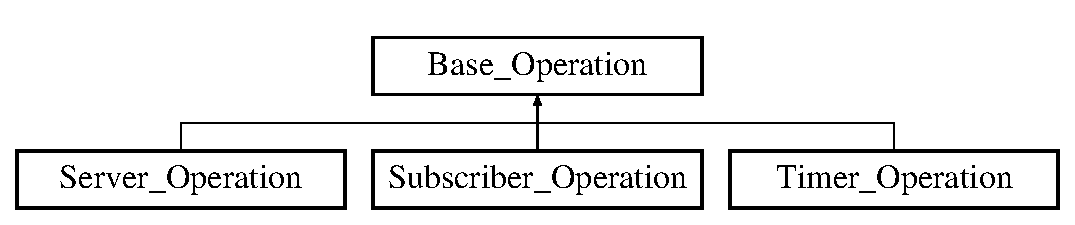
\includegraphics[height=2.000000cm]{classBase__Operation}
\end{center}
\end{figure}
\subsection*{Public Member Functions}
\begin{DoxyCompactItemize}
\item 
{\bfseries Base\+\_\+\+Operation} (std\+::string name, unsigned int priority)\hypertarget{classBase__Operation_a304b48dd7ee48e1010acb5e08cf9bfdf}{}\label{classBase__Operation_a304b48dd7ee48e1010acb5e08cf9bfdf}

\item 
std\+::string {\bfseries get\+\_\+name} ()\hypertarget{classBase__Operation_a878dd0e855a78907e4c828b1d70587d0}{}\label{classBase__Operation_a878dd0e855a78907e4c828b1d70587d0}

\item 
unsigned int {\bfseries get\+\_\+priority} () const \hypertarget{classBase__Operation_a0d561f85d2454f7c5abbe9d0e264a98a}{}\label{classBase__Operation_a0d561f85d2454f7c5abbe9d0e264a98a}

\item 
virtual void {\bfseries execute} ()\hypertarget{classBase__Operation_a79b95449af5927c70e5e243b36a5e250}{}\label{classBase__Operation_a79b95449af5927c70e5e243b36a5e250}

\end{DoxyCompactItemize}


The documentation for this class was generated from the following file\+:\begin{DoxyCompactItemize}
\item 
/home/pranav/\+Repositories/zmq-\/comm/include/operation\+\_\+types.\+hpp\end{DoxyCompactItemize}

\hypertarget{classClient}{}\section{Client Class Reference}
\label{classClient}\index{Client@{Client}}
\subsection*{Public Member Functions}
\begin{DoxyCompactItemize}
\item 
{\bfseries Client} (std\+::string name)\hypertarget{classClient_a3155b89414f2f61ec50d1ba639aa2611}{}\label{classClient_a3155b89414f2f61ec50d1ba639aa2611}

\item 
{\bfseries Client} (std\+::string name, std\+::vector$<$ std\+::string $>$ endpoints)\hypertarget{classClient_a5920215827fbf2dd09f37dddc573d5c9}{}\label{classClient_a5920215827fbf2dd09f37dddc573d5c9}

\item 
void {\bfseries connect} (std\+::vector$<$ std\+::string $>$ new\+\_\+endpoints)\hypertarget{classClient_a24feacb5cf3e55549586fd7b3b3827da}{}\label{classClient_a24feacb5cf3e55549586fd7b3b3827da}

\item 
std\+::string {\bfseries get\+\_\+name} ()\hypertarget{classClient_a159e477ab6a0f0d7e77e5a4426d7de78}{}\label{classClient_a159e477ab6a0f0d7e77e5a4426d7de78}

\item 
std\+::string {\bfseries call} (std\+::string message)\hypertarget{classClient_a5e980004675cbbd1a8b37caf26508ecd}{}\label{classClient_a5e980004675cbbd1a8b37caf26508ecd}

\end{DoxyCompactItemize}


The documentation for this class was generated from the following file\+:\begin{DoxyCompactItemize}
\item 
/home/pranav/\+Repositories/zmq-\/comm/include/client.\+hpp\end{DoxyCompactItemize}

\hypertarget{classComponent}{}\section{Component Class Reference}
\label{classComponent}\index{Component@{Component}}
\subsection*{Public Member Functions}
\begin{DoxyCompactItemize}
\item 
std\+::thread $\ast$ {\bfseries spawn} ()\hypertarget{classComponent_a18c2c6005703233baba1881a301c3c2e}{}\label{classComponent_a18c2c6005703233baba1881a301c3c2e}

\end{DoxyCompactItemize}
\subsection*{Protected Attributes}
\begin{DoxyCompactItemize}
\item 
\hyperlink{classOperation__Queue}{Operation\+\_\+\+Queue} $\ast$ {\bfseries operation\+\_\+queue}\hypertarget{classComponent_a403c5d873156e4933d4bf617e8031b87}{}\label{classComponent_a403c5d873156e4933d4bf617e8031b87}

\item 
std\+::thread $\ast$ {\bfseries executor\+\_\+thread}\hypertarget{classComponent_aba9f6d41585cffa7939b982827659862}{}\label{classComponent_aba9f6d41585cffa7939b982827659862}

\end{DoxyCompactItemize}


The documentation for this class was generated from the following file\+:\begin{DoxyCompactItemize}
\item 
/home/pranav/\+Repositories/zmq-\/comm/include/component.\+hpp\end{DoxyCompactItemize}

\hypertarget{classOperation__Queue}{}\section{Operation\+\_\+\+Queue Class Reference}
\label{classOperation__Queue}\index{Operation\+\_\+\+Queue@{Operation\+\_\+\+Queue}}
\subsection*{Classes}
\begin{DoxyCompactItemize}
\item 
struct \hyperlink{structOperation__Queue_1_1PriorityOrdering}{Priority\+Ordering}
\end{DoxyCompactItemize}
\subsection*{Public Member Functions}
\begin{DoxyCompactItemize}
\item 
void {\bfseries enqueue} (\hyperlink{classBase__Operation}{Base\+\_\+\+Operation} $\ast$new\+\_\+operation)\hypertarget{classOperation__Queue_a5d6e152023fb1397c57943a4335a1d36}{}\label{classOperation__Queue_a5d6e152023fb1397c57943a4335a1d36}

\item 
void {\bfseries dequeue} ()\hypertarget{classOperation__Queue_a56dcc8bb196a32a7d4cf6f657bd4508f}{}\label{classOperation__Queue_a56dcc8bb196a32a7d4cf6f657bd4508f}

\item 
bool {\bfseries empty} ()\hypertarget{classOperation__Queue_ade8aa8ed0a275711f1a2b93495713360}{}\label{classOperation__Queue_ade8aa8ed0a275711f1a2b93495713360}

\item 
\hyperlink{classBase__Operation}{Base\+\_\+\+Operation} $\ast$ {\bfseries top} ()\hypertarget{classOperation__Queue_aae5d94270ca2214abef384dced8f76c0}{}\label{classOperation__Queue_aae5d94270ca2214abef384dced8f76c0}

\item 
void {\bfseries process} ()\hypertarget{classOperation__Queue_ae4b30cda2e2b6f2d33c99a60437d4ffe}{}\label{classOperation__Queue_ae4b30cda2e2b6f2d33c99a60437d4ffe}

\item 
std\+::thread $\ast$ {\bfseries spawn} ()\hypertarget{classOperation__Queue_a05f1899538aa7d4b635e00ad9a66d277}{}\label{classOperation__Queue_a05f1899538aa7d4b635e00ad9a66d277}

\end{DoxyCompactItemize}


The documentation for this class was generated from the following file\+:\begin{DoxyCompactItemize}
\item 
/home/pranav/\+Repositories/zmq-\/comm/include/operation\+\_\+queue.\+hpp\end{DoxyCompactItemize}

\hypertarget{structOperation__Queue_1_1PriorityOrdering}{}\section{Operation\+\_\+\+Queue\+:\+:Priority\+Ordering Struct Reference}
\label{structOperation__Queue_1_1PriorityOrdering}\index{Operation\+\_\+\+Queue\+::\+Priority\+Ordering@{Operation\+\_\+\+Queue\+::\+Priority\+Ordering}}
\subsection*{Public Member Functions}
\begin{DoxyCompactItemize}
\item 
bool {\bfseries operator()} (const \hyperlink{classBase__Operation}{Base\+\_\+\+Operation} $\ast$lhs, const \hyperlink{classBase__Operation}{Base\+\_\+\+Operation} $\ast$rhs) const \hypertarget{structOperation__Queue_1_1PriorityOrdering_a5f707bcd126c09e2c68ac7c79fed3ffd}{}\label{structOperation__Queue_1_1PriorityOrdering_a5f707bcd126c09e2c68ac7c79fed3ffd}

\end{DoxyCompactItemize}


The documentation for this struct was generated from the following file\+:\begin{DoxyCompactItemize}
\item 
/home/pranav/\+Repositories/zmq-\/comm/include/operation\+\_\+queue.\+hpp\end{DoxyCompactItemize}

\hypertarget{classPublisher}{}\section{Publisher Class Reference}
\label{classPublisher}\index{Publisher@{Publisher}}
\subsection*{Public Member Functions}
\begin{DoxyCompactItemize}
\item 
{\bfseries Publisher} (std\+::string name)\hypertarget{classPublisher_a50a9290519fbd4f11aec0577dd4d660a}{}\label{classPublisher_a50a9290519fbd4f11aec0577dd4d660a}

\item 
{\bfseries Publisher} (std\+::string name, std\+::vector$<$ std\+::string $>$ endpoints)\hypertarget{classPublisher_ac65d758b8bf78e6b8e03dd2842862362}{}\label{classPublisher_ac65d758b8bf78e6b8e03dd2842862362}

\item 
void {\bfseries bind} (std\+::vector$<$ std\+::string $>$ new\+\_\+endpoints)\hypertarget{classPublisher_ae87340722160ca793e63efafef895869}{}\label{classPublisher_ae87340722160ca793e63efafef895869}

\item 
std\+::string {\bfseries get\+\_\+name} ()\hypertarget{classPublisher_a0987adfed11685e41bb899e10551efa3}{}\label{classPublisher_a0987adfed11685e41bb899e10551efa3}

\item 
void {\bfseries add\+\_\+connection} (std\+::string new\+\_\+connection)\hypertarget{classPublisher_a18ec9ed7e62a781adfaeaaf30e585f83}{}\label{classPublisher_a18ec9ed7e62a781adfaeaaf30e585f83}

\item 
void {\bfseries send} (std\+::string message)\hypertarget{classPublisher_a23c145dcf3aa27de262c2c5a2e947b26}{}\label{classPublisher_a23c145dcf3aa27de262c2c5a2e947b26}

\end{DoxyCompactItemize}


The documentation for this class was generated from the following file\+:\begin{DoxyCompactItemize}
\item 
/home/pranav/\+Repositories/zmq-\/comm/include/publisher.\+hpp\end{DoxyCompactItemize}

\hypertarget{classServer}{}\section{Server Class Reference}
\label{classServer}\index{Server@{Server}}
\subsection*{Public Member Functions}
\begin{DoxyCompactItemize}
\item 
{\bfseries Server} (std\+::string name, unsigned int priority, std\+::function$<$ std\+::string(const std\+::string \&)$>$ operation\+\_\+function, \hyperlink{classOperation__Queue}{Operation\+\_\+\+Queue} $\ast$operation\+\_\+queue\+\_\+ptr)\hypertarget{classServer_a1e77c9c5b6fbc63b023ac083efd8c6ea}{}\label{classServer_a1e77c9c5b6fbc63b023ac083efd8c6ea}

\item 
{\bfseries Server} (std\+::string name, unsigned int priority, std\+::vector$<$ std\+::string $>$ endpoints, std\+::function$<$ std\+::string(const std\+::string \&)$>$ operation\+\_\+function, \hyperlink{classOperation__Queue}{Operation\+\_\+\+Queue} $\ast$operation\+\_\+queue\+\_\+ptr)\hypertarget{classServer_a6c8e865c9e8a488719f10e106abc75be}{}\label{classServer_a6c8e865c9e8a488719f10e106abc75be}

\item 
void {\bfseries bind} (std\+::vector$<$ std\+::string $>$ new\+\_\+endpoints)\hypertarget{classServer_a25286f8ab603f3cd7bd76842f2a8b78d}{}\label{classServer_a25286f8ab603f3cd7bd76842f2a8b78d}

\item 
std\+::string {\bfseries get\+\_\+name} ()\hypertarget{classServer_a09d72bd75643ee43dea39a4753d6df05}{}\label{classServer_a09d72bd75643ee43dea39a4753d6df05}

\item 
unsigned int {\bfseries get\+\_\+priority} ()\hypertarget{classServer_a1c7613df4abf1aaf59b709ad4b3ed8a3}{}\label{classServer_a1c7613df4abf1aaf59b709ad4b3ed8a3}

\item 
void {\bfseries add\+\_\+connection} (std\+::string new\+\_\+connection)\hypertarget{classServer_a71256b14e081575403eefbb6aa6c08bf}{}\label{classServer_a71256b14e081575403eefbb6aa6c08bf}

\item 
void {\bfseries recv} ()\hypertarget{classServer_a6bb73ef31c7ed34fad165435b581d7a9}{}\label{classServer_a6bb73ef31c7ed34fad165435b581d7a9}

\item 
void {\bfseries rebind\+\_\+operation\+\_\+function} (std\+::function$<$ std\+::string(const std\+::string \&)$>$ new\+\_\+operation\+\_\+function)\hypertarget{classServer_add9087ce6bbe672d22d4d80565696653}{}\label{classServer_add9087ce6bbe672d22d4d80565696653}

\item 
std\+::thread {\bfseries spawn} ()\hypertarget{classServer_afaa5fab09f6a4582ae4b29232ebd9f76}{}\label{classServer_afaa5fab09f6a4582ae4b29232ebd9f76}

\item 
void {\bfseries start} ()\hypertarget{classServer_a7eac07d2582fa01c2671362efa955b31}{}\label{classServer_a7eac07d2582fa01c2671362efa955b31}

\end{DoxyCompactItemize}


The documentation for this class was generated from the following file\+:\begin{DoxyCompactItemize}
\item 
/home/pranav/\+Repositories/zmq-\/comm/include/server.\+hpp\end{DoxyCompactItemize}

\hypertarget{classServer__Operation}{}\section{Server\+\_\+\+Operation Class Reference}
\label{classServer__Operation}\index{Server\+\_\+\+Operation@{Server\+\_\+\+Operation}}
Inheritance diagram for Server\+\_\+\+Operation\+:\begin{figure}[H]
\begin{center}
\leavevmode
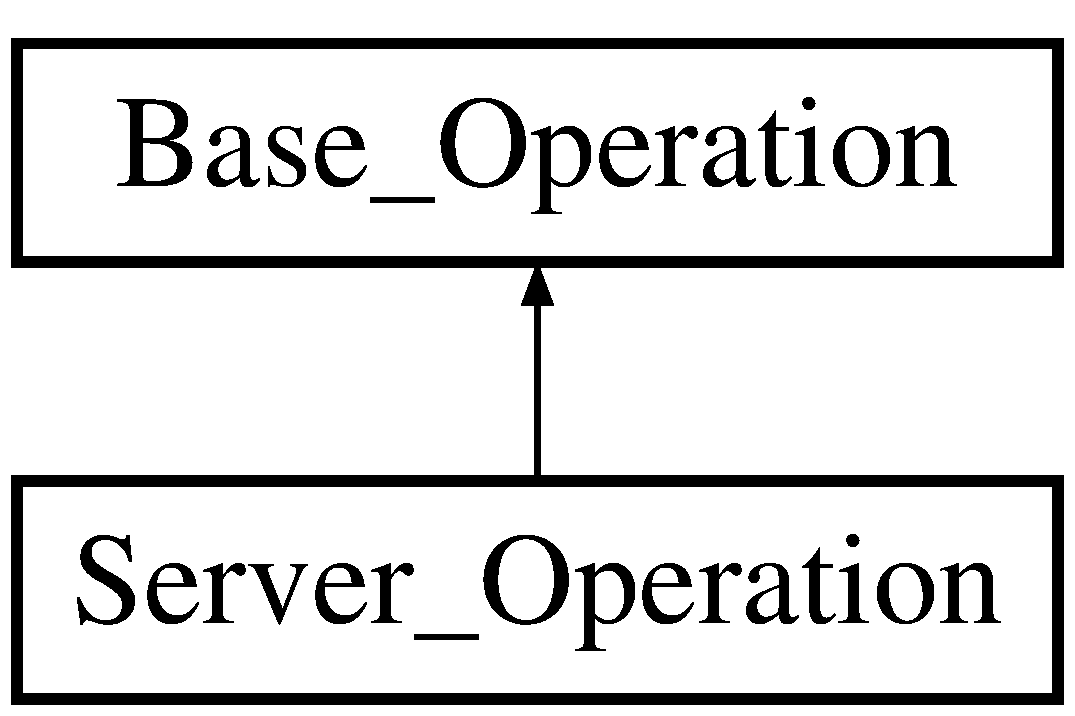
\includegraphics[height=2.000000cm]{classServer__Operation}
\end{center}
\end{figure}
\subsection*{Public Member Functions}
\begin{DoxyCompactItemize}
\item 
{\bfseries Server\+\_\+\+Operation} (std\+::string name, unsigned int priority, std\+::function$<$ std\+::string()$>$ operation\+\_\+function, zmq\+::socket\+\_\+t $\ast$socket\+\_\+ptr, bool $\ast$recv\+\_\+ready)\hypertarget{classServer__Operation_a2f23da94de8bbec78ed8ed31a10bc59e}{}\label{classServer__Operation_a2f23da94de8bbec78ed8ed31a10bc59e}

\item 
void {\bfseries execute} ()\hypertarget{classServer__Operation_a5f9fd79477344d73687d6b566e6b9a02}{}\label{classServer__Operation_a5f9fd79477344d73687d6b566e6b9a02}

\item 
zmq\+::socket\+\_\+t $\ast$ {\bfseries get\+\_\+socket\+\_\+ptr} ()\hypertarget{classServer__Operation_a6209f8ceaf75bbdbf7a9d1666fc07957}{}\label{classServer__Operation_a6209f8ceaf75bbdbf7a9d1666fc07957}

\item 
void {\bfseries set\+\_\+ready} ()\hypertarget{classServer__Operation_a47b181b85afb6f791128c34b6ebefc3b}{}\label{classServer__Operation_a47b181b85afb6f791128c34b6ebefc3b}

\item 
std\+::string {\bfseries get\+\_\+name} ()\hypertarget{classBase__Operation_a878dd0e855a78907e4c828b1d70587d0}{}\label{classBase__Operation_a878dd0e855a78907e4c828b1d70587d0}

\item 
unsigned int {\bfseries get\+\_\+priority} () const \hypertarget{classBase__Operation_a0d561f85d2454f7c5abbe9d0e264a98a}{}\label{classBase__Operation_a0d561f85d2454f7c5abbe9d0e264a98a}

\end{DoxyCompactItemize}


The documentation for this class was generated from the following file\+:\begin{DoxyCompactItemize}
\item 
/home/pranav/\+Repositories/zmq-\/comm/include/operation\+\_\+types.\+hpp\end{DoxyCompactItemize}

\hypertarget{classSubscriber}{}\section{Subscriber Class Reference}
\label{classSubscriber}\index{Subscriber@{Subscriber}}
\subsection*{Public Member Functions}
\begin{DoxyCompactItemize}
\item 
{\bfseries Subscriber} (std\+::string name, unsigned int priority, std\+::string filter, std\+::function$<$ void(const std\+::string \&)$>$ operation\+\_\+function, \hyperlink{classOperation__Queue}{Operation\+\_\+\+Queue} $\ast$operation\+\_\+queue\+\_\+ptr)\hypertarget{classSubscriber_a21da7eaa648e01d062e73318fb7efa1c}{}\label{classSubscriber_a21da7eaa648e01d062e73318fb7efa1c}

\item 
{\bfseries Subscriber} (std\+::string name, unsigned int priority, std\+::string filter, std\+::vector$<$ std\+::string $>$ endpoints, std\+::function$<$ void(const std\+::string \&)$>$ operation\+\_\+function, \hyperlink{classOperation__Queue}{Operation\+\_\+\+Queue} $\ast$operation\+\_\+queue\+\_\+ptr)\hypertarget{classSubscriber_aa24c82c7bfe2754c4220f38e93fd820f}{}\label{classSubscriber_aa24c82c7bfe2754c4220f38e93fd820f}

\item 
void {\bfseries connect} (std\+::vector$<$ std\+::string $>$ new\+\_\+endpoints)\hypertarget{classSubscriber_ac5f15d5b5b17723a806fc0c3d27cc0d9}{}\label{classSubscriber_ac5f15d5b5b17723a806fc0c3d27cc0d9}

\item 
std\+::string {\bfseries get\+\_\+name} ()\hypertarget{classSubscriber_aaaca14d4fe5aab6ea77cb8e1d3514fbe}{}\label{classSubscriber_aaaca14d4fe5aab6ea77cb8e1d3514fbe}

\item 
unsigned int {\bfseries get\+\_\+priority} ()\hypertarget{classSubscriber_aeb42dbfd280972f49cc7878b1508f1d5}{}\label{classSubscriber_aeb42dbfd280972f49cc7878b1508f1d5}

\item 
void {\bfseries add\+\_\+connection} (std\+::string new\+\_\+connection)\hypertarget{classSubscriber_ae9a7c65672dd0a8ae94af8ade499e8c1}{}\label{classSubscriber_ae9a7c65672dd0a8ae94af8ade499e8c1}

\item 
void {\bfseries recv} ()\hypertarget{classSubscriber_a9f11c50282c4c6b3d0f13e7509e12cf4}{}\label{classSubscriber_a9f11c50282c4c6b3d0f13e7509e12cf4}

\item 
void {\bfseries rebind\+\_\+operation\+\_\+function} (std\+::function$<$ void(const std\+::string \&)$>$ new\+\_\+operation\+\_\+function)\hypertarget{classSubscriber_accb8f931d762a94aee12f2c5f8b892c7}{}\label{classSubscriber_accb8f931d762a94aee12f2c5f8b892c7}

\item 
std\+::thread {\bfseries spawn} ()\hypertarget{classSubscriber_a67e14a76406e393f4448f18558cb93f8}{}\label{classSubscriber_a67e14a76406e393f4448f18558cb93f8}

\item 
void {\bfseries start} ()\hypertarget{classSubscriber_a9299f928c18fbdb444f624be47a7cf69}{}\label{classSubscriber_a9299f928c18fbdb444f624be47a7cf69}

\end{DoxyCompactItemize}


The documentation for this class was generated from the following file\+:\begin{DoxyCompactItemize}
\item 
/home/pranav/\+Repositories/zmq-\/comm/include/subscriber.\+hpp\end{DoxyCompactItemize}

\hypertarget{classSubscriber__Operation}{}\section{Subscriber\+\_\+\+Operation Class Reference}
\label{classSubscriber__Operation}\index{Subscriber\+\_\+\+Operation@{Subscriber\+\_\+\+Operation}}
Inheritance diagram for Subscriber\+\_\+\+Operation\+:\begin{figure}[H]
\begin{center}
\leavevmode
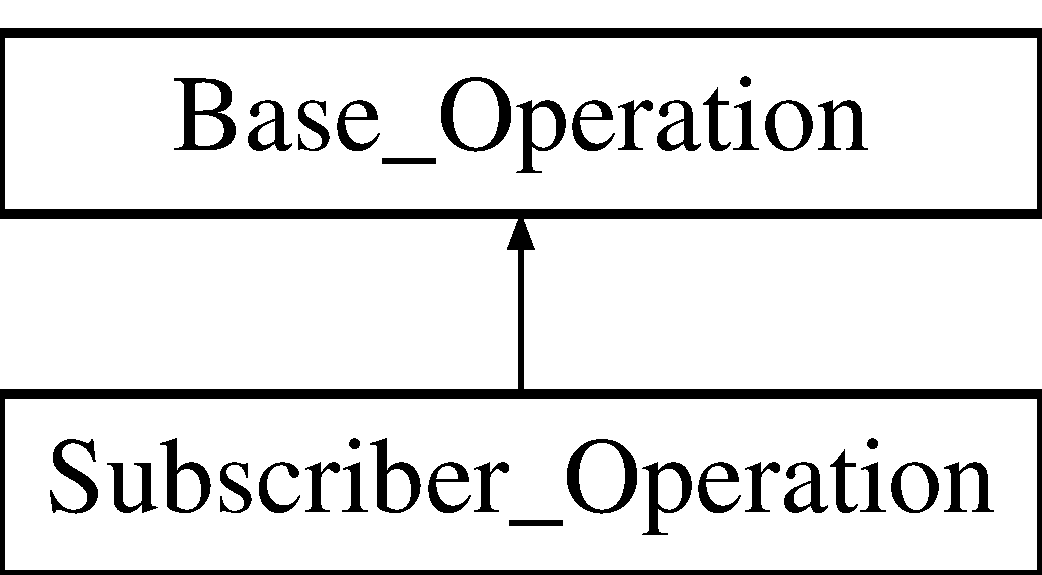
\includegraphics[height=2.000000cm]{classSubscriber__Operation}
\end{center}
\end{figure}
\subsection*{Public Member Functions}
\begin{DoxyCompactItemize}
\item 
{\bfseries Subscriber\+\_\+\+Operation} (std\+::string name, unsigned int priority, std\+::function$<$ void()$>$ operation\+\_\+function)\hypertarget{classSubscriber__Operation_a12cd9532aec72e1a5c2264ef9bf854af}{}\label{classSubscriber__Operation_a12cd9532aec72e1a5c2264ef9bf854af}

\item 
void {\bfseries execute} ()\hypertarget{classSubscriber__Operation_a8163faae3d4f4a05c0279dcf63112909}{}\label{classSubscriber__Operation_a8163faae3d4f4a05c0279dcf63112909}

\item 
std\+::string {\bfseries get\+\_\+name} ()\hypertarget{classBase__Operation_a878dd0e855a78907e4c828b1d70587d0}{}\label{classBase__Operation_a878dd0e855a78907e4c828b1d70587d0}

\item 
unsigned int {\bfseries get\+\_\+priority} () const \hypertarget{classBase__Operation_a0d561f85d2454f7c5abbe9d0e264a98a}{}\label{classBase__Operation_a0d561f85d2454f7c5abbe9d0e264a98a}

\end{DoxyCompactItemize}


The documentation for this class was generated from the following file\+:\begin{DoxyCompactItemize}
\item 
/home/pranav/\+Repositories/zmq-\/comm/include/operation\+\_\+types.\+hpp\end{DoxyCompactItemize}

\hypertarget{classTimer}{}\section{Timer Class Reference}
\label{classTimer}\index{Timer@{Timer}}


\hyperlink{classTimer}{Timer} class.  




{\ttfamily \#include $<$timer.\+hpp$>$}

\subsection*{Public Member Functions}
\begin{DoxyCompactItemize}
\item 
{\bfseries Timer} (std\+::string name, unsigned int priority, long long period, std\+::function$<$ void()$>$ operation\+\_\+function, \hyperlink{classOperation__Queue}{Operation\+\_\+\+Queue} $\ast$operation\+\_\+queue\+\_\+ptr)\hypertarget{classTimer_a16df63cd14ab5d1b4239283babd27e30}{}\label{classTimer_a16df63cd14ab5d1b4239283babd27e30}

\item 
void {\bfseries operation} ()\hypertarget{classTimer_a0210f7f3f1ce0999a469a04c0fd202ac}{}\label{classTimer_a0210f7f3f1ce0999a469a04c0fd202ac}

\item 
std\+::string {\bfseries get\+\_\+name} ()\hypertarget{classTimer_a19255976397d5af980913b314aee1b9c}{}\label{classTimer_a19255976397d5af980913b314aee1b9c}

\item 
unsigned int {\bfseries get\+\_\+priority} ()\hypertarget{classTimer_ae10e24cb90e19951244503465738e745}{}\label{classTimer_ae10e24cb90e19951244503465738e745}

\item 
void {\bfseries change\+\_\+period} (long long new\+\_\+period)\hypertarget{classTimer_a871ff84116553c144bb3416743125fb8}{}\label{classTimer_a871ff84116553c144bb3416743125fb8}

\item 
void {\bfseries rebind\+\_\+operation\+\_\+function} (std\+::function$<$ void()$>$ new\+\_\+operation\+\_\+function)\hypertarget{classTimer_ad6efdb8f9a9be1d0bd2ca3786f5d1166}{}\label{classTimer_ad6efdb8f9a9be1d0bd2ca3786f5d1166}

\item 
std\+::thread {\bfseries spawn} ()\hypertarget{classTimer_a6d7dc6419b2eac8dec4997097ec5a2dd}{}\label{classTimer_a6d7dc6419b2eac8dec4997097ec5a2dd}

\item 
void {\bfseries start} ()\hypertarget{classTimer_a3a8b5272198d029779dc9302a54305a8}{}\label{classTimer_a3a8b5272198d029779dc9302a54305a8}

\end{DoxyCompactItemize}


\subsection{Detailed Description}
\hyperlink{classTimer}{Timer} class. 

The documentation for this class was generated from the following files\+:\begin{DoxyCompactItemize}
\item 
/home/pranav/\+Repositories/zmq-\/comm/include/\hyperlink{timer_8hpp}{timer.\+hpp}\item 
/home/pranav/\+Repositories/zmq-\/comm/src/\hyperlink{timer_8cpp}{timer.\+cpp}\end{DoxyCompactItemize}

\hypertarget{classTimer__Operation}{}\section{Timer\+\_\+\+Operation Class Reference}
\label{classTimer__Operation}\index{Timer\+\_\+\+Operation@{Timer\+\_\+\+Operation}}
Inheritance diagram for Timer\+\_\+\+Operation\+:\begin{figure}[H]
\begin{center}
\leavevmode
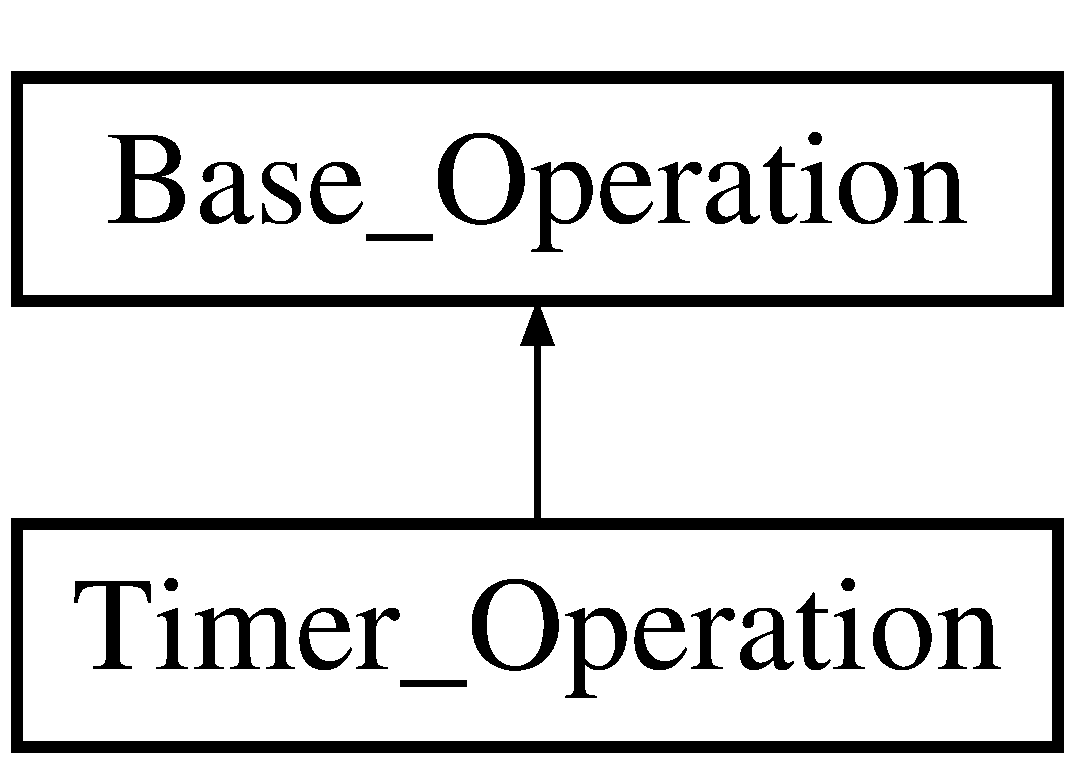
\includegraphics[height=2.000000cm]{classTimer__Operation}
\end{center}
\end{figure}
\subsection*{Public Member Functions}
\begin{DoxyCompactItemize}
\item 
{\bfseries Timer\+\_\+\+Operation} (std\+::string name, unsigned int priority, std\+::function$<$ void()$>$ operation\+\_\+function)\hypertarget{classTimer__Operation_ac964edca7ceffca9d55b081e0142ac8a}{}\label{classTimer__Operation_ac964edca7ceffca9d55b081e0142ac8a}

\item 
void {\bfseries execute} ()\hypertarget{classTimer__Operation_a9d20628449efe98de6628c7bd03d4dd4}{}\label{classTimer__Operation_a9d20628449efe98de6628c7bd03d4dd4}

\item 
std\+::string {\bfseries get\+\_\+name} ()\hypertarget{classBase__Operation_a878dd0e855a78907e4c828b1d70587d0}{}\label{classBase__Operation_a878dd0e855a78907e4c828b1d70587d0}

\item 
unsigned int {\bfseries get\+\_\+priority} () const \hypertarget{classBase__Operation_a0d561f85d2454f7c5abbe9d0e264a98a}{}\label{classBase__Operation_a0d561f85d2454f7c5abbe9d0e264a98a}

\end{DoxyCompactItemize}


The documentation for this class was generated from the following file\+:\begin{DoxyCompactItemize}
\item 
/home/pranav/\+Repositories/zmq-\/comm/include/operation\+\_\+types.\+hpp\end{DoxyCompactItemize}

\hypertarget{classXML__Parser}{}\section{X\+M\+L\+\_\+\+Parser Class Reference}
\label{classXML__Parser}\index{X\+M\+L\+\_\+\+Parser@{X\+M\+L\+\_\+\+Parser}}
\subsection*{Public Member Functions}
\begin{DoxyCompactItemize}
\item 
{\bfseries X\+M\+L\+\_\+\+Parser} (const char $\ast$filename)\hypertarget{classXML__Parser_aa0a4bad8139300742b2458f81f171d7f}{}\label{classXML__Parser_aa0a4bad8139300742b2458f81f171d7f}

\item 
void {\bfseries parse} ()\hypertarget{classXML__Parser_ae8f40d4faba09275a2d2e97c8966c379}{}\label{classXML__Parser_ae8f40d4faba09275a2d2e97c8966c379}

\end{DoxyCompactItemize}


The documentation for this class was generated from the following file\+:\begin{DoxyCompactItemize}
\item 
/home/pranav/\+Repositories/zmq-\/comm/include/xml\+\_\+parser.\+hpp\end{DoxyCompactItemize}

\chapter{File Documentation}
\hypertarget{timer_8hpp}{\section{/home/kelsier/\-Git\-Hub/zcm/include/timer.hpp File Reference}
\label{timer_8hpp}\index{/home/kelsier/\-Git\-Hub/zcm/include/timer.\-hpp@{/home/kelsier/\-Git\-Hub/zcm/include/timer.\-hpp}}
}


This file declares the Timer class.  


{\ttfamily \#include $<$iostream$>$}\\*
{\ttfamily \#include $<$string$>$}\\*
{\ttfamily \#include $<$chrono$>$}\\*
{\ttfamily \#include $<$ratio$>$}\\*
{\ttfamily \#include $<$thread$>$}\\*
{\ttfamily \#include \char`\"{}operation\-\_\-queue.\-hpp\char`\"{}}\\*
\subsection*{Classes}
\begin{DoxyCompactItemize}
\item 
class \hyperlink{classzcm_1_1Timer}{zcm\-::\-Timer}
\begin{DoxyCompactList}\small\item\em \hyperlink{classzcm_1_1Timer}{Timer} class. \end{DoxyCompactList}\end{DoxyCompactItemize}
\subsection*{Namespaces}
\begin{DoxyCompactItemize}
\item 
\hyperlink{namespacezcm}{zcm}
\end{DoxyCompactItemize}


\subsection{Detailed Description}
This file declares the Timer class. \begin{DoxyAuthor}{Author}
Pranav Srinivas Kumar 
\end{DoxyAuthor}
\begin{DoxyDate}{Date}
2016.\-04.\-24 
\end{DoxyDate}

\hypertarget{timer_8cpp}{}\section{/home/pranav/\+Repositories/zmq-\/comm/src/timer.cpp File Reference}
\label{timer_8cpp}\index{/home/pranav/\+Repositories/zmq-\/comm/src/timer.\+cpp@{/home/pranav/\+Repositories/zmq-\/comm/src/timer.\+cpp}}


This file contains definitions for the \hyperlink{classTimer}{Timer} class.  


{\ttfamily \#include \char`\"{}timer.\+hpp\char`\"{}}\\*


\subsection{Detailed Description}
This file contains definitions for the \hyperlink{classTimer}{Timer} class. 

\begin{DoxyAuthor}{Author}
Pranav Srinivas Kumar 
\end{DoxyAuthor}
\begin{DoxyDate}{Date}
2016.\+04.\+24 
\end{DoxyDate}

%--- End generated contents ---

% Index
\backmatter
\newpage
\phantomsection
\clearemptydoublepage
\addcontentsline{toc}{chapter}{Index}
\printindex

\end{document}
